\documentclass[1p]{elsarticle_modified}
%\bibliographystyle{elsarticle-num}

%\usepackage[colorlinks]{hyperref}
%\usepackage{abbrmath_seonhwa} %\Abb, \Ascr, \Acal ,\Abf, \Afrak
\usepackage{amsfonts}
\usepackage{amssymb}
\usepackage{amsmath}
\usepackage{amsthm}
\usepackage{scalefnt}
\usepackage{amsbsy}
\usepackage{kotex}
\usepackage{caption}
\usepackage{subfig}
\usepackage{color}
\usepackage{graphicx}
\usepackage{xcolor} %% white, black, red, green, blue, cyan, magenta, yellow
\usepackage{float}
\usepackage{setspace}
\usepackage{hyperref}

\usepackage{tikz}
\usetikzlibrary{arrows}

\usepackage{multirow}
\usepackage{array} % fixed length table
\usepackage{hhline}

%%%%%%%%%%%%%%%%%%%%%
\makeatletter
\renewcommand*\env@matrix[1][\arraystretch]{%
	\edef\arraystretch{#1}%
	\hskip -\arraycolsep
	\let\@ifnextchar\new@ifnextchar
	\array{*\c@MaxMatrixCols c}}
\makeatother %https://tex.stackexchange.com/questions/14071/how-can-i-increase-the-line-spacing-in-a-matrix
%%%%%%%%%%%%%%%

\usepackage[normalem]{ulem}

\newcommand{\msout}[1]{\ifmmode\text{\sout{\ensuremath{#1}}}\else\sout{#1}\fi}
%SOURCE: \msout is \stkout macro in https://tex.stackexchange.com/questions/20609/strikeout-in-math-mode

\newcommand{\cancel}[1]{
	\ifmmode
	{\color{red}\msout{#1}}
	\else
	{\color{red}\sout{#1}}
	\fi
}

\newcommand{\add}[1]{
	{\color{blue}\uwave{#1}}
}

\newcommand{\replace}[2]{
	\ifmmode
	{\color{red}\msout{#1}}{\color{blue}\uwave{#2}}
	\else
	{\color{red}\sout{#1}}{\color{blue}\uwave{#2}}
	\fi
}

\newcommand{\Sol}{\mathcal{S}} %segment
\newcommand{\D}{D} %diagram
\newcommand{\A}{\mathcal{A}} %arc


%%%%%%%%%%%%%%%%%%%%%%%%%%%%%5 test

\def\sl{\operatorname{\textup{SL}}(2,\Cbb)}
\def\psl{\operatorname{\textup{PSL}}(2,\Cbb)}
\def\quan{\mkern 1mu \triangleright \mkern 1mu}

\theoremstyle{definition}
\newtheorem{thm}{Theorem}[section]
\newtheorem{prop}[thm]{Proposition}
\newtheorem{lem}[thm]{Lemma}
\newtheorem{ques}[thm]{Question}
\newtheorem{cor}[thm]{Corollary}
\newtheorem{defn}[thm]{Definition}
\newtheorem{exam}[thm]{Example}
\newtheorem{rmk}[thm]{Remark}
\newtheorem{alg}[thm]{Algorithm}

\newcommand{\I}{\sqrt{-1}}
\begin{document}

%\begin{frontmatter}
%
%\title{Boundary parabolic representations of knots up to 8 crossings}
%
%%% Group authors per affiliation:
%\author{Yunhi Cho} 
%\address{Department of Mathematics, University of Seoul, Seoul, Korea}
%\ead{yhcho@uos.ac.kr}
%
%
%\author{Seonhwa Kim} %\fnref{s_kim}}
%\address{Center for Geometry and Physics, Institute for Basic Science, Pohang, 37673, Korea}
%\ead{ryeona17@ibs.re.kr}
%
%\author{Hyuk Kim}
%\address{Department of Mathematical Sciences, Seoul National University, Seoul 08826, Korea}
%\ead{hyukkim@snu.ac.kr}
%
%\author{Seokbeom Yoon}
%\address{Department of Mathematical Sciences, Seoul National University, Seoul, 08826,  Korea}
%\ead{sbyoon15@snu.ac.kr}
%
%\begin{abstract}
%We find all boundary parabolic representation of knots up to 8 crossings.
%
%\end{abstract}
%\begin{keyword}
%    \MSC[2010] 57M25 
%\end{keyword}
%
%\end{frontmatter}

%\linenumbers
%\tableofcontents
%
\newcommand\colored[1]{\textcolor{white}{\rule[-0.35ex]{0.8em}{1.4ex}}\kern-0.8em\color{red} #1}%
%\newcommand\colored[1]{\textcolor{white}{ #1}\kern-2.17ex	\textcolor{white}{ #1}\kern-1.81ex	\textcolor{white}{ #1}\kern-2.15ex\color{red}#1	}

{\Large $\underline{12n_{0437}~(K12n_{0437})}$}

\setlength{\tabcolsep}{10pt}
\renewcommand{\arraystretch}{1.6}
\vspace{1cm}\begin{tabular}{m{100pt}>{\centering\arraybackslash}m{274pt}}
\multirow{5}{120pt}{
	\centering
	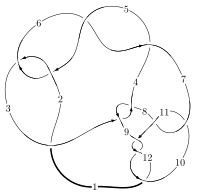
\includegraphics[width=112pt]{../../../GIT/diagram.site/Diagrams/png/2526_12n_0437.png}\\
\ \ \ A knot diagram\footnotemark}&
\allowdisplaybreaks
\textbf{Linearized knot diagam} \\
\cline{2-2}
 &
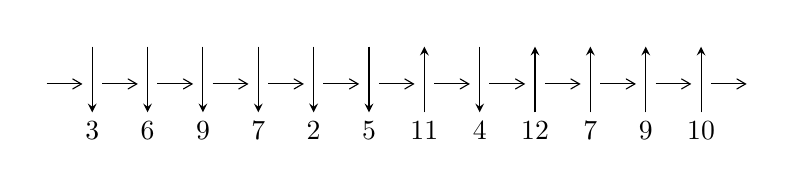
\begin{tikzpicture}[x=20pt, y=17pt]
	% nodes
	\node (C0) at (0, 0) {};
	\node (C1) at (1, 0) {};
	\node (C1U) at (1, +1) {};
	\node (C1D) at (1, -1) {3};

	\node (C2) at (2, 0) {};
	\node (C2U) at (2, +1) {};
	\node (C2D) at (2, -1) {6};

	\node (C3) at (3, 0) {};
	\node (C3U) at (3, +1) {};
	\node (C3D) at (3, -1) {9};

	\node (C4) at (4, 0) {};
	\node (C4U) at (4, +1) {};
	\node (C4D) at (4, -1) {7};

	\node (C5) at (5, 0) {};
	\node (C5U) at (5, +1) {};
	\node (C5D) at (5, -1) {2};

	\node (C6) at (6, 0) {};
	\node (C6U) at (6, +1) {};
	\node (C6D) at (6, -1) {5};

	\node (C7) at (7, 0) {};
	\node (C7U) at (7, +1) {};
	\node (C7D) at (7, -1) {11};

	\node (C8) at (8, 0) {};
	\node (C8U) at (8, +1) {};
	\node (C8D) at (8, -1) {4};

	\node (C9) at (9, 0) {};
	\node (C9U) at (9, +1) {};
	\node (C9D) at (9, -1) {12};

	\node (C10) at (10, 0) {};
	\node (C10U) at (10, +1) {};
	\node (C10D) at (10, -1) {7};

	\node (C11) at (11, 0) {};
	\node (C11U) at (11, +1) {};
	\node (C11D) at (11, -1) {9};

	\node (C12) at (12, 0) {};
	\node (C12U) at (12, +1) {};
	\node (C12D) at (12, -1) {10};
	\node (C13) at (13, 0) {};

	% arrows
	\draw[->,>={angle 60}]
	(C0) edge (C1) (C1) edge (C2) (C2) edge (C3) (C3) edge (C4) (C4) edge (C5) (C5) edge (C6) (C6) edge (C7) (C7) edge (C8) (C8) edge (C9) (C9) edge (C10) (C10) edge (C11) (C11) edge (C12) (C12) edge (C13) ;	\draw[->,>=stealth]
	(C1U) edge (C1D) (C2U) edge (C2D) (C3U) edge (C3D) (C4U) edge (C4D) (C5U) edge (C5D) (C6U) edge (C6D) (C7D) edge (C7U) (C8U) edge (C8D) (C9D) edge (C9U) (C10D) edge (C10U) (C11D) edge (C11U) (C12D) edge (C12U) ;
	\end{tikzpicture} \\
\hhline{~~} \\& 
\textbf{Solving Sequence} \\ \cline{2-2} 
 &
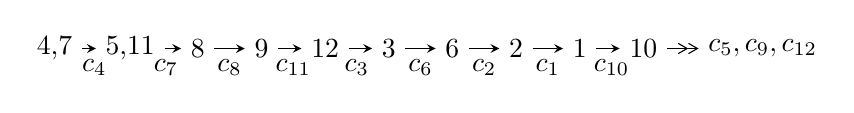
\begin{tikzpicture}[x=23pt, y=7pt]
	% node
	\node (A0) at (-1/8, 0) {4,7};
	\node (A1) at (17/16, 0) {5,11};
	\node (A2) at (17/8, 0) {8};
	\node (A3) at (25/8, 0) {9};
	\node (A4) at (33/8, 0) {12};
	\node (A5) at (41/8, 0) {3};
	\node (A6) at (49/8, 0) {6};
	\node (A7) at (57/8, 0) {2};
	\node (A8) at (65/8, 0) {1};
	\node (A9) at (73/8, 0) {10};
	\node (C1) at (1/2, -1) {$c_{4}$};
	\node (C2) at (13/8, -1) {$c_{7}$};
	\node (C3) at (21/8, -1) {$c_{8}$};
	\node (C4) at (29/8, -1) {$c_{11}$};
	\node (C5) at (37/8, -1) {$c_{3}$};
	\node (C6) at (45/8, -1) {$c_{6}$};
	\node (C7) at (53/8, -1) {$c_{2}$};
	\node (C8) at (61/8, -1) {$c_{1}$};
	\node (C9) at (69/8, -1) {$c_{10}$};
	\node (A10) at (11, 0) {$c_{5},c_{9},c_{12}$};

	% edge
	\draw[->,>=stealth]	
	(A0) edge (A1) (A1) edge (A2) (A2) edge (A3) (A3) edge (A4) (A4) edge (A5) (A5) edge (A6) (A6) edge (A7) (A7) edge (A8) (A8) edge (A9) ;
	\draw[->>,>={angle 60}]	
	(A9) edge (A10);
\end{tikzpicture} \\ 

\end{tabular} \\

\footnotetext{
The image of knot diagram is generated by the software ``\textbf{Draw programme}" developed by Andrew Bartholomew(\url{http://www.layer8.co.uk/maths/draw/index.htm\#Running-draw}), where we modified some parts for our purpose(\url{https://github.com/CATsTAILs/LinksPainter}).
}\phantom \\ \newline 
\centering \textbf{Ideals for irreducible components\footnotemark of $X_{\text{par}}$} 
 
\begin{align*}
I^u_{1}&=\langle 
9.19324\times10^{24} u^{24}-9.37535\times10^{25} u^{23}+\cdots+7.01855\times10^{25} b+8.63495\times10^{25},\\
\phantom{I^u_{1}}&\phantom{= \langle  }-4.13470\times10^{25} u^{24}+4.13261\times10^{26} u^{23}+\cdots+7.01855\times10^{25} a-2.79968\times10^{27},\\
\phantom{I^u_{1}}&\phantom{= \langle  }u^{25}-10 u^{24}+\cdots+72 u-1\rangle \\
I^u_{2}&=\langle 
- u^4+u^3-4 u^2+b+3 u-3,\;a,\;u^5- u^4+4 u^3-3 u^2+3 u-1\rangle \\
I^u_{3}&=\langle 
u^2 a+b+u,\;u^2 a+a^2- a u-2 u^2+2 a+u-3,\;u^3- u^2+2 u-1\rangle \\
\\
\end{align*}
\raggedright * 3 irreducible components of $\dim_{\mathbb{C}}=0$, with total 36 representations.\\
\footnotetext{All coefficients of polynomials are rational numbers. But the coefficients are sometimes approximated in decimal forms when there is not enough margin.}
\newpage
\renewcommand{\arraystretch}{1}
\centering \section*{I. $I^u_{1}= \langle 9.19\times10^{24} u^{24}-9.38\times10^{25} u^{23}+\cdots+7.02\times10^{25} b+8.63\times10^{25},\;-4.13\times10^{25} u^{24}+4.13\times10^{26} u^{23}+\cdots+7.02\times10^{25} a-2.80\times10^{27},\;u^{25}-10 u^{24}+\cdots+72 u-1 \rangle$}
\flushleft \textbf{(i) Arc colorings}\\
\begin{tabular}{m{7pt} m{180pt} m{7pt} m{180pt} }
\flushright $a_{4}=$&$\begin{pmatrix}1\\0\end{pmatrix}$ \\
\flushright $a_{7}=$&$\begin{pmatrix}0\\u\end{pmatrix}$ \\
\flushright $a_{5}=$&$\begin{pmatrix}1\\u^2\end{pmatrix}$ \\
\flushright $a_{11}=$&$\begin{pmatrix}0.589110 u^{24}-5.88812 u^{23}+\cdots-335.813 u+39.8897\\-0.130985 u^{24}+1.33580 u^{23}+\cdots+39.4166 u-1.23030\end{pmatrix}$ \\
\flushright $a_{8}=$&$\begin{pmatrix}0.452645 u^{24}-4.39464 u^{23}+\cdots-195.754 u+22.1379\\-0.146274 u^{24}+1.40258 u^{23}+\cdots+20.5478 u-0.642297\end{pmatrix}$ \\
\flushright $a_{9}=$&$\begin{pmatrix}0.598919 u^{24}-5.79722 u^{23}+\cdots-216.301 u+22.7802\\-0.146274 u^{24}+1.40258 u^{23}+\cdots+20.5478 u-0.642297\end{pmatrix}$ \\
\flushright $a_{12}=$&$\begin{pmatrix}0.598919 u^{24}-5.79722 u^{23}+\cdots-216.301 u+22.7802\\0.0345873 u^{24}-0.219643 u^{23}+\cdots+21.9603 u-0.710241\end{pmatrix}$ \\
\flushright $a_{3}=$&$\begin{pmatrix}-0.0157966 u^{24}+0.0835882 u^{23}+\cdots-49.3795 u+8.57675\\-0.0421281 u^{24}+0.395025 u^{23}+\cdots+1.19935 u-0.137223\end{pmatrix}$ \\
\flushright $a_{6}=$&$\begin{pmatrix}u\\u^3+u\end{pmatrix}$ \\
\flushright $a_{2}=$&$\begin{pmatrix}0.0628449 u^{24}-0.637985 u^{23}+\cdots-55.7029 u+8.66493\\0.0743783 u^{24}-0.692119 u^{23}+\cdots-9.71411 u+0.0157966\end{pmatrix}$ \\
\flushright $a_{1}=$&$\begin{pmatrix}0.137223 u^{24}-1.33010 u^{23}+\cdots-65.4171 u+8.68072\\0.100634 u^{24}-0.951779 u^{23}+\cdots-12.6101 u+0.0579248\end{pmatrix}$ \\
\flushright $a_{10}=$&$\begin{pmatrix}0.589110 u^{24}-5.88812 u^{23}+\cdots-335.813 u+39.8897\\-0.137742 u^{24}+1.39067 u^{23}+\cdots+39.7915 u-1.22733\end{pmatrix}$\\&\end{tabular}
\flushleft \textbf{(ii) Obstruction class $= -1$}\\~\\
\flushleft \textbf{(iii) Cusp Shapes $= \frac{25106355762453601367160863}{23395155619836929736818172} u^{24}-\frac{62945700046644877607050528}{5848788904959232434204543} u^{23}+\cdots-\frac{511603421605188008732954519}{1376185624696289984518716} u+\frac{351161482484964948702456565}{23395155619836929736818172}$}\\~\\
\newpage\renewcommand{\arraystretch}{1}
\flushleft \textbf{(iv) u-Polynomials at the component}\newline \\
\begin{tabular}{m{50pt}|m{274pt}}
Crossings & \hspace{64pt}u-Polynomials at each crossing \\
\hline $$\begin{aligned}c_{1},c_{4},c_{6}\end{aligned}$$&$\begin{aligned}
&u^{25}+10 u^{24}+\cdots+72 u+1
\end{aligned}$\\
\hline $$\begin{aligned}c_{2},c_{5}\end{aligned}$$&$\begin{aligned}
&u^{25}+4 u^{24}+\cdots-12 u-1
\end{aligned}$\\
\hline $$\begin{aligned}c_{3},c_{8}\end{aligned}$$&$\begin{aligned}
&u^{25}-2 u^{24}+\cdots-32 u-64
\end{aligned}$\\
\hline $$\begin{aligned}c_{7},c_{10}\end{aligned}$$&$\begin{aligned}
&u^{25}-4 u^{24}+\cdots-192 u-32
\end{aligned}$\\
\hline $$\begin{aligned}c_{9},c_{11},c_{12}\end{aligned}$$&$\begin{aligned}
&u^{25}+9 u^{24}+\cdots-41 u+1
\end{aligned}$\\
\hline
\end{tabular}\\~\\
\newpage\renewcommand{\arraystretch}{1}
\flushleft \textbf{(v) Riley Polynomials at the component}\newline \\
\begin{tabular}{m{50pt}|m{274pt}}
Crossings & \hspace{64pt}Riley Polynomials at each crossing \\
\hline $$\begin{aligned}c_{1},c_{4},c_{6}\end{aligned}$$&$\begin{aligned}
&y^{25}+14 y^{24}+\cdots+4016 y-1
\end{aligned}$\\
\hline $$\begin{aligned}c_{2},c_{5}\end{aligned}$$&$\begin{aligned}
&y^{25}-10 y^{24}+\cdots+72 y-1
\end{aligned}$\\
\hline $$\begin{aligned}c_{3},c_{8}\end{aligned}$$&$\begin{aligned}
&y^{25}-28 y^{24}+\cdots+29696 y-4096
\end{aligned}$\\
\hline $$\begin{aligned}c_{7},c_{10}\end{aligned}$$&$\begin{aligned}
&y^{25}+24 y^{24}+\cdots+51712 y-1024
\end{aligned}$\\
\hline $$\begin{aligned}c_{9},c_{11},c_{12}\end{aligned}$$&$\begin{aligned}
&y^{25}-9 y^{24}+\cdots+1947 y-1
\end{aligned}$\\
\hline
\end{tabular}\\~\\
\newpage\flushleft \textbf{(vi) Complex Volumes and Cusp Shapes}
$$\begin{array}{c|c|c}  
\text{Solutions to }I^u_{1}& \I (\text{vol} + \sqrt{-1}CS) & \text{Cusp shape}\\
 \hline 
\begin{aligned}
u &= -0.799543 + 0.627415 I \\
a &= -0.93941 + 1.56370 I \\
b &= -0.01758 + 1.51331 I\end{aligned}
 & -4.36096 - 1.13139 I & \phantom{-}0.75657 + 1.52598 I \\ \hline\begin{aligned}
u &= -0.799543 - 0.627415 I \\
a &= -0.93941 - 1.56370 I \\
b &= -0.01758 - 1.51331 I\end{aligned}
 & -4.36096 + 1.13139 I & \phantom{-}0.75657 - 1.52598 I \\ \hline\begin{aligned}
u &= -0.034202 + 0.923614 I \\
a &= -0.686187 - 0.237402 I \\
b &= \phantom{-}0.108494 + 0.547445 I\end{aligned}
 & \phantom{-}1.97950 - 1.66008 I & -0.69040 + 2.96263 I \\ \hline\begin{aligned}
u &= -0.034202 - 0.923614 I \\
a &= -0.686187 + 0.237402 I \\
b &= \phantom{-}0.108494 - 0.547445 I\end{aligned}
 & \phantom{-}1.97950 + 1.66008 I & -0.69040 - 2.96263 I \\ \hline\begin{aligned}
u &= \phantom{-}0.856820 + 0.829058 I \\
a &= \phantom{-}1.063360 - 0.668986 I \\
b &= \phantom{-}0.022399 - 0.950691 I\end{aligned}
 & -0.38972 - 2.81828 I & -1.13877 + 3.80627 I \\ \hline\begin{aligned}
u &= \phantom{-}0.856820 - 0.829058 I \\
a &= \phantom{-}1.063360 + 0.668986 I \\
b &= \phantom{-}0.022399 + 0.950691 I\end{aligned}
 & -0.38972 + 2.81828 I & -1.13877 - 3.80627 I \\ \hline\begin{aligned}
u &= \phantom{-}0.755262\phantom{ +0.000000I} \\
a &= -2.29591\phantom{ +0.000000I} \\
b &= \phantom{-}0.108132\phantom{ +0.000000I}\end{aligned}
 & \phantom{-}7.52575\phantom{ +0.000000I} & -13.1500\phantom{ +0.000000I} \\ \hline\begin{aligned}
u &= \phantom{-}0.240993 + 1.276750 I \\
a &= -0.034747 + 0.379118 I \\
b &= \phantom{-}0.13663 + 3.40519 I\end{aligned}
 & \phantom{-}4.24524 - 2.77554 I & \phantom{-}34.2342 + 3.0457 I \\ \hline\begin{aligned}
u &= \phantom{-}0.240993 - 1.276750 I \\
a &= -0.034747 - 0.379118 I \\
b &= \phantom{-}0.13663 - 3.40519 I\end{aligned}
 & \phantom{-}4.24524 + 2.77554 I & \phantom{-}34.2342 - 3.0457 I \\ \hline\begin{aligned}
u &= -0.563738 + 1.206990 I \\
a &= \phantom{-}0.839591 - 1.130370 I \\
b &= -0.40514 - 1.62951 I\end{aligned}
 & -2.40018 + 6.37988 I & \phantom{-}2.18378 - 2.52933 I\\
 \hline 
 \end{array}$$\newpage$$\begin{array}{c|c|c}  
\text{Solutions to }I^u_{1}& \I (\text{vol} + \sqrt{-1}CS) & \text{Cusp shape}\\
 \hline 
\begin{aligned}
u &= -0.563738 - 1.206990 I \\
a &= \phantom{-}0.839591 + 1.130370 I \\
b &= -0.40514 + 1.62951 I\end{aligned}
 & -2.40018 - 6.37988 I & \phantom{-}2.18378 + 2.52933 I \\ \hline\begin{aligned}
u &= \phantom{-}0.75670 + 1.19685 I \\
a &= \phantom{-}0.860055 + 0.001764 I \\
b &= -0.149981 + 0.594534 I\end{aligned}
 & \phantom{-}0.73025 - 3.27384 I & -1.24326 + 3.27643 I \\ \hline\begin{aligned}
u &= \phantom{-}0.75670 - 1.19685 I \\
a &= \phantom{-}0.860055 - 0.001764 I \\
b &= -0.149981 - 0.594534 I\end{aligned}
 & \phantom{-}0.73025 + 3.27384 I & -1.24326 - 3.27643 I \\ \hline\begin{aligned}
u &= \phantom{-}0.462757 + 0.342084 I \\
a &= -0.172877 - 1.143600 I \\
b &= -0.66811 - 1.47469 I\end{aligned}
 & \phantom{-}0.902564 - 0.255949 I & -3.12150 + 6.64716 I \\ \hline\begin{aligned}
u &= \phantom{-}0.462757 - 0.342084 I \\
a &= -0.172877 + 1.143600 I \\
b &= -0.66811 + 1.47469 I\end{aligned}
 & \phantom{-}0.902564 + 0.255949 I & -3.12150 - 6.64716 I \\ \hline\begin{aligned}
u &= \phantom{-}0.447970\phantom{ +0.000000I} \\
a &= -0.336060\phantom{ +0.000000I} \\
b &= \phantom{-}0.456804\phantom{ +0.000000I}\end{aligned}
 & -0.908338\phantom{ +0.000000I} & -11.6550\phantom{ +0.000000I} \\ \hline\begin{aligned}
u &= \phantom{-}0.11903 + 1.59221 I \\
a &= -0.113155 + 0.609313 I \\
b &= \phantom{-}0.018929 + 0.249452 I\end{aligned}
 & \phantom{-}13.29460 - 3.19957 I & \phantom{-}9.89238 + 1.87771 I \\ \hline\begin{aligned}
u &= \phantom{-}0.11903 - 1.59221 I \\
a &= -0.113155 - 0.609313 I \\
b &= \phantom{-}0.018929 - 0.249452 I\end{aligned}
 & \phantom{-}13.29460 + 3.19957 I & \phantom{-}9.89238 - 1.87771 I \\ \hline\begin{aligned}
u &= \phantom{-}1.63956 + 0.34345 I \\
a &= -0.019703 - 1.413500 I \\
b &= \phantom{-}0.15371 - 1.68285 I\end{aligned}
 & -10.18570 - 4.57384 I & \phantom{-0.000000 -}0. + 2.62009 I \\ \hline\begin{aligned}
u &= \phantom{-}1.63956 - 0.34345 I \\
a &= -0.019703 + 1.413500 I \\
b &= \phantom{-}0.15371 + 1.68285 I\end{aligned}
 & -10.18570 + 4.57384 I & \phantom{-0.000000 } 0. - 2.62009 I\\
 \hline 
 \end{array}$$\newpage$$\begin{array}{c|c|c}  
\text{Solutions to }I^u_{1}& \I (\text{vol} + \sqrt{-1}CS) & \text{Cusp shape}\\
 \hline 
\begin{aligned}
u &= \phantom{-}1.04678 + 1.44405 I \\
a &= \phantom{-}0.689190 + 1.046230 I \\
b &= -0.09880 + 1.59912 I\end{aligned}
 & -7.03225 - 4.52109 I & \phantom{-0.000000 } 0 \\ \hline\begin{aligned}
u &= \phantom{-}1.04678 - 1.44405 I \\
a &= \phantom{-}0.689190 - 1.046230 I \\
b &= -0.09880 - 1.59912 I\end{aligned}
 & -7.03225 + 4.52109 I & \phantom{-0.000000 } 0 \\ \hline\begin{aligned}
u &= \phantom{-}0.66532 + 1.68962 I \\
a &= -0.626781 - 0.927153 I \\
b &= \phantom{-}0.44778 - 1.73312 I\end{aligned}
 & -3.94520 - 12.71920 I & \phantom{-0.000000 } 0 \\ \hline\begin{aligned}
u &= \phantom{-}0.66532 - 1.68962 I \\
a &= -0.626781 + 0.927153 I \\
b &= \phantom{-}0.44778 + 1.73312 I\end{aligned}
 & -3.94520 + 12.71920 I & \phantom{-0.000000 } 0 \\ \hline\begin{aligned}
u &= \phantom{-}0.0157871\phantom{ +0.000000I} \\
a &= \phantom{-}34.9133\phantom{ +0.000000I} \\
b &= -0.661595\phantom{ +0.000000I}\end{aligned}
 & \phantom{-}1.12664\phantom{ +0.000000I} & \phantom{-}9.59670\phantom{ +0.000000I}\\
 \hline 
 \end{array}$$\newpage\newpage\renewcommand{\arraystretch}{1}
\centering \section*{II. $I^u_{2}= \langle - u^4+u^3-4 u^2+b+3 u-3,\;a,\;u^5- u^4+4 u^3-3 u^2+3 u-1 \rangle$}
\flushleft \textbf{(i) Arc colorings}\\
\begin{tabular}{m{7pt} m{180pt} m{7pt} m{180pt} }
\flushright $a_{4}=$&$\begin{pmatrix}1\\0\end{pmatrix}$ \\
\flushright $a_{7}=$&$\begin{pmatrix}0\\u\end{pmatrix}$ \\
\flushright $a_{5}=$&$\begin{pmatrix}1\\u^2\end{pmatrix}$ \\
\flushright $a_{11}=$&$\begin{pmatrix}0\\u^4- u^3+4 u^2-3 u+3\end{pmatrix}$ \\
\flushright $a_{8}=$&$\begin{pmatrix}0\\u\end{pmatrix}$ \\
\flushright $a_{9}=$&$\begin{pmatrix}- u\\u\end{pmatrix}$ \\
\flushright $a_{12}=$&$\begin{pmatrix}u\\u^4- u^3+4 u^2-4 u+3\end{pmatrix}$ \\
\flushright $a_{3}=$&$\begin{pmatrix}u^2+1\\- u^2\end{pmatrix}$ \\
\flushright $a_{6}=$&$\begin{pmatrix}u\\u^3+u\end{pmatrix}$ \\
\flushright $a_{2}=$&$\begin{pmatrix}u^3+2 u\\- u^3- u\end{pmatrix}$ \\
\flushright $a_{1}=$&$\begin{pmatrix}u\\- u\end{pmatrix}$ \\
\flushright $a_{10}=$&$\begin{pmatrix}0\\u^4- u^3+4 u^2-3 u+3\end{pmatrix}$\\&\end{tabular}
\flushleft \textbf{(ii) Obstruction class $= 1$}\\~\\
\flushleft \textbf{(iii) Cusp Shapes $= -18 u^4+11 u^3-65 u^2+29 u-38$}\\~\\
\newpage\renewcommand{\arraystretch}{1}
\flushleft \textbf{(iv) u-Polynomials at the component}\newline \\
\begin{tabular}{m{50pt}|m{274pt}}
Crossings & \hspace{64pt}u-Polynomials at each crossing \\
\hline $$\begin{aligned}c_{1},c_{3},c_{4}\end{aligned}$$&$\begin{aligned}
&u^5- u^4+4 u^3-3 u^2+3 u-1
\end{aligned}$\\
\hline $$\begin{aligned}c_{2}\end{aligned}$$&$\begin{aligned}
&u^5- u^4+u^2+u-1
\end{aligned}$\\
\hline $$\begin{aligned}c_{5}\end{aligned}$$&$\begin{aligned}
&u^5+u^4- u^2+u+1
\end{aligned}$\\
\hline $$\begin{aligned}c_{6},c_{8}\end{aligned}$$&$\begin{aligned}
&u^5+u^4+4 u^3+3 u^2+3 u+1
\end{aligned}$\\
\hline $$\begin{aligned}c_{7},c_{10}\end{aligned}$$&$\begin{aligned}
&u^5
\end{aligned}$\\
\hline $$\begin{aligned}c_{9}\end{aligned}$$&$\begin{aligned}
&(u+1)^5
\end{aligned}$\\
\hline $$\begin{aligned}c_{11},c_{12}\end{aligned}$$&$\begin{aligned}
&(u-1)^5
\end{aligned}$\\
\hline
\end{tabular}\\~\\
\newpage\renewcommand{\arraystretch}{1}
\flushleft \textbf{(v) Riley Polynomials at the component}\newline \\
\begin{tabular}{m{50pt}|m{274pt}}
Crossings & \hspace{64pt}Riley Polynomials at each crossing \\
\hline $$\begin{aligned}c_{1},c_{3},c_{4}\\c_{6},c_{8}\end{aligned}$$&$\begin{aligned}
&y^5+7 y^4+16 y^3+13 y^2+3 y-1
\end{aligned}$\\
\hline $$\begin{aligned}c_{2},c_{5}\end{aligned}$$&$\begin{aligned}
&y^5- y^4+4 y^3-3 y^2+3 y-1
\end{aligned}$\\
\hline $$\begin{aligned}c_{7},c_{10}\end{aligned}$$&$\begin{aligned}
&y^5
\end{aligned}$\\
\hline $$\begin{aligned}c_{9},c_{11},c_{12}\end{aligned}$$&$\begin{aligned}
&(y-1)^5
\end{aligned}$\\
\hline
\end{tabular}\\~\\
\newpage\flushleft \textbf{(vi) Complex Volumes and Cusp Shapes}
$$\begin{array}{c|c|c}  
\text{Solutions to }I^u_{2}& \I (\text{vol} + \sqrt{-1}CS) & \text{Cusp shape}\\
 \hline 
\begin{aligned}
u &= \phantom{-}0.233677 + 0.885557 I \\
a &= \phantom{-0.000000 } 0 \\
b &= \phantom{-}0.278580 - 1.055720 I\end{aligned}
 & \phantom{-}3.46474 - 2.21397 I & \phantom{-}3.79538 + 3.60694 I \\ \hline\begin{aligned}
u &= \phantom{-}0.233677 - 0.885557 I \\
a &= \phantom{-0.000000 } 0 \\
b &= \phantom{-}0.278580 + 1.055720 I\end{aligned}
 & \phantom{-}3.46474 + 2.21397 I & \phantom{-}3.79538 - 3.60694 I \\ \hline\begin{aligned}
u &= \phantom{-}0.416284\phantom{ +0.000000I} \\
a &= \phantom{-0.000000 } 0 \\
b &= \phantom{-}2.40221\phantom{ +0.000000I}\end{aligned}
 & \phantom{-}0.762751\phantom{ +0.000000I} & -36.9390\phantom{ +0.000000I} \\ \hline\begin{aligned}
u &= \phantom{-}0.05818 + 1.69128 I \\
a &= \phantom{-0.000000 } 0 \\
b &= \phantom{-}0.020316 - 0.590570 I\end{aligned}
 & \phantom{-}12.60320 - 3.33174 I & -2.32599 + 3.47010 I \\ \hline\begin{aligned}
u &= \phantom{-}0.05818 - 1.69128 I \\
a &= \phantom{-0.000000 } 0 \\
b &= \phantom{-}0.020316 + 0.590570 I\end{aligned}
 & \phantom{-}12.60320 + 3.33174 I & -2.32599 - 3.47010 I\\
 \hline 
 \end{array}$$\newpage\newpage\renewcommand{\arraystretch}{1}
\centering \section*{III. $I^u_{3}= \langle u^2 a+b+u,\;u^2 a+a^2- a u-2 u^2+2 a+u-3,\;u^3- u^2+2 u-1 \rangle$}
\flushleft \textbf{(i) Arc colorings}\\
\begin{tabular}{m{7pt} m{180pt} m{7pt} m{180pt} }
\flushright $a_{4}=$&$\begin{pmatrix}1\\0\end{pmatrix}$ \\
\flushright $a_{7}=$&$\begin{pmatrix}0\\u\end{pmatrix}$ \\
\flushright $a_{5}=$&$\begin{pmatrix}1\\u^2\end{pmatrix}$ \\
\flushright $a_{11}=$&$\begin{pmatrix}a\\- u^2 a- u\end{pmatrix}$ \\
\flushright $a_{8}=$&$\begin{pmatrix}u^2- a- u+2\\0\end{pmatrix}$ \\
\flushright $a_{9}=$&$\begin{pmatrix}u^2- a- u+2\\0\end{pmatrix}$ \\
\flushright $a_{12}=$&$\begin{pmatrix}u^2- a- u+2\\- u^2 a- u\end{pmatrix}$ \\
\flushright $a_{3}=$&$\begin{pmatrix}1\\0\end{pmatrix}$ \\
\flushright $a_{6}=$&$\begin{pmatrix}u\\u^2- u+1\end{pmatrix}$ \\
\flushright $a_{2}=$&$\begin{pmatrix}u\\- u\end{pmatrix}$ \\
\flushright $a_{1}=$&$\begin{pmatrix}0\\- u\end{pmatrix}$ \\
\flushright $a_{10}=$&$\begin{pmatrix}a\\- u\end{pmatrix}$\\&\end{tabular}
\flushleft \textbf{(ii) Obstruction class $= 1$}\\~\\
\flushleft \textbf{(iii) Cusp Shapes $= -3 a u+5 u^2-3 a+2 u+4$}\\~\\
\newpage\renewcommand{\arraystretch}{1}
\flushleft \textbf{(iv) u-Polynomials at the component}\newline \\
\begin{tabular}{m{50pt}|m{274pt}}
Crossings & \hspace{64pt}u-Polynomials at each crossing \\
\hline $$\begin{aligned}c_{1},c_{4}\end{aligned}$$&$\begin{aligned}
&(u^3- u^2+2 u-1)^2
\end{aligned}$\\
\hline $$\begin{aligned}c_{2}\end{aligned}$$&$\begin{aligned}
&(u^3+u^2-1)^2
\end{aligned}$\\
\hline $$\begin{aligned}c_{3},c_{8}\end{aligned}$$&$\begin{aligned}
&u^6
\end{aligned}$\\
\hline $$\begin{aligned}c_{5}\end{aligned}$$&$\begin{aligned}
&(u^3- u^2+1)^2
\end{aligned}$\\
\hline $$\begin{aligned}c_{6}\end{aligned}$$&$\begin{aligned}
&(u^3+u^2+2 u+1)^2
\end{aligned}$\\
\hline $$\begin{aligned}c_{7},c_{9}\end{aligned}$$&$\begin{aligned}
&(u^2- u-1)^3
\end{aligned}$\\
\hline $$\begin{aligned}c_{10},c_{11},c_{12}\end{aligned}$$&$\begin{aligned}
&(u^2+u-1)^3
\end{aligned}$\\
\hline
\end{tabular}\\~\\
\newpage\renewcommand{\arraystretch}{1}
\flushleft \textbf{(v) Riley Polynomials at the component}\newline \\
\begin{tabular}{m{50pt}|m{274pt}}
Crossings & \hspace{64pt}Riley Polynomials at each crossing \\
\hline $$\begin{aligned}c_{1},c_{4},c_{6}\end{aligned}$$&$\begin{aligned}
&(y^3+3 y^2+2 y-1)^2
\end{aligned}$\\
\hline $$\begin{aligned}c_{2},c_{5}\end{aligned}$$&$\begin{aligned}
&(y^3- y^2+2 y-1)^2
\end{aligned}$\\
\hline $$\begin{aligned}c_{3},c_{8}\end{aligned}$$&$\begin{aligned}
&y^6
\end{aligned}$\\
\hline $$\begin{aligned}c_{7},c_{9},c_{10}\\c_{11},c_{12}\end{aligned}$$&$\begin{aligned}
&(y^2-3 y+1)^3
\end{aligned}$\\
\hline
\end{tabular}\\~\\
\newpage\flushleft \textbf{(vi) Complex Volumes and Cusp Shapes}
$$\begin{array}{c|c|c}  
\text{Solutions to }I^u_{3}& \I (\text{vol} + \sqrt{-1}CS) & \text{Cusp shape}\\
 \hline 
\begin{aligned}
u &= \phantom{-}0.215080 + 1.307140 I \\
a &= -0.198308 + 1.205210 I \\
b &= \phantom{-}0.132927 + 0.807858 I\end{aligned}
 & \phantom{-}11.90680 - 2.82812 I & \phantom{-}1.56739 + 1.81005 I \\ \hline\begin{aligned}
u &= \phantom{-}0.215080 + 1.307140 I \\
a &= \phantom{-}0.075747 - 0.460350 I \\
b &= -0.34801 - 2.11500 I\end{aligned}
 & \phantom{-}4.01109 - 2.82812 I & -5.96298 + 6.80673 I \\ \hline\begin{aligned}
u &= \phantom{-}0.215080 - 1.307140 I \\
a &= -0.198308 - 1.205210 I \\
b &= \phantom{-}0.132927 - 0.807858 I\end{aligned}
 & \phantom{-}11.90680 + 2.82812 I & \phantom{-}1.56739 - 1.81005 I \\ \hline\begin{aligned}
u &= \phantom{-}0.215080 - 1.307140 I \\
a &= \phantom{-}0.075747 + 0.460350 I \\
b &= -0.34801 + 2.11500 I\end{aligned}
 & \phantom{-}4.01109 + 2.82812 I & -5.96298 - 6.80673 I \\ \hline\begin{aligned}
u &= \phantom{-}0.569840\phantom{ +0.000000I} \\
a &= \phantom{-}1.08457\phantom{ +0.000000I} \\
b &= -0.922021\phantom{ +0.000000I}\end{aligned}
 & -0.126494\phantom{ +0.000000I} & \phantom{-}1.65540\phantom{ +0.000000I} \\ \hline\begin{aligned}
u &= \phantom{-}0.569840\phantom{ +0.000000I} \\
a &= -2.83945\phantom{ +0.000000I} \\
b &= \phantom{-}0.352181\phantom{ +0.000000I}\end{aligned}
 & \phantom{-}7.76919\phantom{ +0.000000I} & \phantom{-}20.1360\phantom{ +0.000000I}\\
 \hline 
 \end{array}$$\newpage
\newpage\renewcommand{\arraystretch}{1}
\centering \section*{ IV. u-Polynomials}
\begin{tabular}{m{50pt}|m{274pt}}
Crossings & \hspace{64pt}u-Polynomials at each crossing \\
\hline $$\begin{aligned}c_{1},c_{4}\end{aligned}$$&$\begin{aligned}
&(u^3- u^2+2 u-1)^2(u^5- u^4+4 u^3-3 u^2+3 u-1)\\
&\cdot(u^{25}+10 u^{24}+\cdots+72 u+1)
\end{aligned}$\\
\hline $$\begin{aligned}c_{2}\end{aligned}$$&$\begin{aligned}
&((u^3+u^2-1)^2)(u^5- u^4+u^2+u-1)(u^{25}+4 u^{24}+\cdots-12 u-1)
\end{aligned}$\\
\hline $$\begin{aligned}c_{3}\end{aligned}$$&$\begin{aligned}
&u^6(u^5- u^4+\cdots+3 u-1)(u^{25}-2 u^{24}+\cdots-32 u-64)
\end{aligned}$\\
\hline $$\begin{aligned}c_{5}\end{aligned}$$&$\begin{aligned}
&((u^3- u^2+1)^2)(u^5+u^4- u^2+u+1)(u^{25}+4 u^{24}+\cdots-12 u-1)
\end{aligned}$\\
\hline $$\begin{aligned}c_{6}\end{aligned}$$&$\begin{aligned}
&(u^3+u^2+2 u+1)^2(u^5+u^4+4 u^3+3 u^2+3 u+1)\\
&\cdot(u^{25}+10 u^{24}+\cdots+72 u+1)
\end{aligned}$\\
\hline $$\begin{aligned}c_{7}\end{aligned}$$&$\begin{aligned}
&u^5(u^2- u-1)^3(u^{25}-4 u^{24}+\cdots-192 u-32)
\end{aligned}$\\
\hline $$\begin{aligned}c_{8}\end{aligned}$$&$\begin{aligned}
&u^6(u^5+u^4+\cdots+3 u+1)(u^{25}-2 u^{24}+\cdots-32 u-64)
\end{aligned}$\\
\hline $$\begin{aligned}c_{9}\end{aligned}$$&$\begin{aligned}
&((u+1)^5)(u^2- u-1)^3(u^{25}+9 u^{24}+\cdots-41 u+1)
\end{aligned}$\\
\hline $$\begin{aligned}c_{10}\end{aligned}$$&$\begin{aligned}
&u^5(u^2+u-1)^3(u^{25}-4 u^{24}+\cdots-192 u-32)
\end{aligned}$\\
\hline $$\begin{aligned}c_{11},c_{12}\end{aligned}$$&$\begin{aligned}
&((u-1)^5)(u^2+u-1)^3(u^{25}+9 u^{24}+\cdots-41 u+1)
\end{aligned}$\\
\hline
\end{tabular}\newpage\renewcommand{\arraystretch}{1}
\centering \section*{ V. Riley Polynomials}
\begin{tabular}{m{50pt}|m{274pt}}
Crossings & \hspace{64pt}Riley Polynomials at each crossing \\
\hline $$\begin{aligned}c_{1},c_{4},c_{6}\end{aligned}$$&$\begin{aligned}
&(y^3+3 y^2+2 y-1)^2(y^5+7 y^4+16 y^3+13 y^2+3 y-1)\\
&\cdot(y^{25}+14 y^{24}+\cdots+4016 y-1)
\end{aligned}$\\
\hline $$\begin{aligned}c_{2},c_{5}\end{aligned}$$&$\begin{aligned}
&(y^3- y^2+2 y-1)^2(y^5- y^4+4 y^3-3 y^2+3 y-1)\\
&\cdot(y^{25}-10 y^{24}+\cdots+72 y-1)
\end{aligned}$\\
\hline $$\begin{aligned}c_{3},c_{8}\end{aligned}$$&$\begin{aligned}
&y^6(y^5+7 y^4+16 y^3+13 y^2+3 y-1)\\
&\cdot(y^{25}-28 y^{24}+\cdots+29696 y-4096)
\end{aligned}$\\
\hline $$\begin{aligned}c_{7},c_{10}\end{aligned}$$&$\begin{aligned}
&y^5(y^2-3 y+1)^3(y^{25}+24 y^{24}+\cdots+51712 y-1024)
\end{aligned}$\\
\hline $$\begin{aligned}c_{9},c_{11},c_{12}\end{aligned}$$&$\begin{aligned}
&((y-1)^5)(y^2-3 y+1)^3(y^{25}-9 y^{24}+\cdots+1947 y-1)
\end{aligned}$\\
\hline
\end{tabular}
\vskip 2pc
\end{document}